\documentclass[border=3pt]{standalone}
\usepackage{tikz}
\usetikzlibrary{arrows.meta,calc}
\tikzset{pin/.style={-{Stealth[length=5pt]}},
  blk/.style={draw, thick, minimum width=24mm, minimum height=26mm, font=\sffamily\small}}
\begin{document}
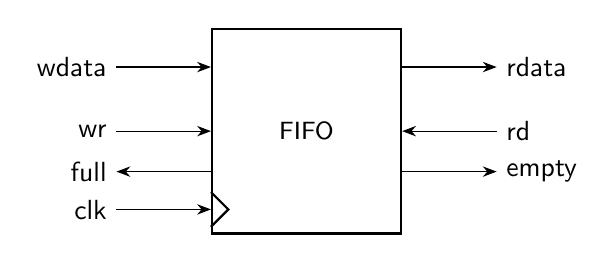
\begin{tikzpicture}[font=\sffamily]
  \node[blk] (f) {FIFO};
  \draw[thick] ($(f.south west)+(0,1mm)$) -- ++(2.2mm,2.2mm) -- ++(-2.2mm,2.2mm);
  % write side (left)
  \draw[pin] ($(f.north west)+(-12mm,-5mm)$) node[left]{wdata} -- ($(f.north west)+(0,-5mm)$);
  \draw[pin] ($(f.west)+(-12mm,0)$) node[left]{wr} -- (f.west);
  \draw[pin] ($(f.south west)+(0,8mm)$) -- ++(-12mm,0) node[left]{full};
  % read side (right)
  \draw[pin] ($(f.north east)+(0,-5mm)$) -- ++(12mm,0) node[right]{rdata};
  \draw[pin] ($(f.east)+(12mm,0)$) node[right]{rd} -- (f.east);
  \draw[pin] ($(f.south east)+(0,8mm)$) -- ++(12mm,0) node[right]{empty};
  \draw[pin] ($(f.south west)+(-12mm,3.2mm)$) node[left]{clk} -- ($(f.south west)+(0,3.2mm)$);
\end{tikzpicture}
\end{document}
